\documentclass{beamer}
\usetheme{metropolis}
\usepackage{graphicx}
\usepackage{subfig}
\usepackage{tcolorbox}
\title{Algebra-Based Physics-2: Electricity, Magnetism, and Modern Physics (PHYS135B-01): Unit 1}
\author{Jordan Hanson}
\institute{Whittier College Department of Physics and Astronomy}

\begin{document}
\maketitle

\section{Summary}

\begin{frame}{Unit 1 Summary}
\textbf{Reading: Chapters 18 and 19}
\begin{enumerate}
\item Charge, mass, the Coulomb force, and the gravitational force
\item Force fields
\item Electric potential and capacitance
\end{enumerate}
\end{frame}

\begin{frame}{Some applications to Biology}
\begin{figure}
\centering
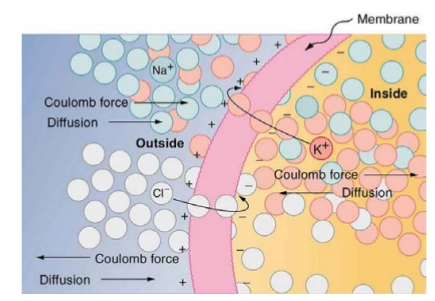
\includegraphics[width=0.6\textwidth]{figures/membrane.png}
\caption{\label{fig:membrane} The cell membrane creates a voltage.}
\end{figure}
\end{frame}

\section{Capacitance}

\begin{frame}{Capacitance}
What voltage is required to store $Q$? Let $\Delta V$ be the voltage difference, $E$ be the electric field strength, and $\Delta x$ be the voltage between the plates.  We already know that
\begin{equation}
\Delta V = E\Delta x
\end{equation}
\textit{But we also know from Coulomb's Law that}
\begin{equation}
E = \frac{\sigma}{\epsilon_0} = \frac{Q}{\epsilon_0 A}
\end{equation}
So we have
\begin{align}
\Delta V &= \frac{Q}{\epsilon_0 A}\Delta x \\
Q &= \left( \frac{\epsilon_0 A}{\Delta x} \right) \Delta V
\end{align}
So now we know how much charge to expect for a given voltage.  The term in parentheses is called \textit{the capacitance, C.}
\end{frame}

\begin{frame}{Capacitance}
Let the capacitor have an area $A$, and plate separation $d$.  The capacitance is
\begin{equation}
\boxed{
C = \frac{\epsilon_0 A}{d}}
\end{equation}
\textit{Capacitance} epresents the ability to store charge.  The unit of capacitance is \textbf{the farad}, after Michael Faraday (encounter mid-semester).  Scaling problems in a moment...
\end{frame}

\section{PhET Activity: Capacitor Basics}

\begin{frame}
\small
Go to the activity: \\ \vspace{0.5cm}
\url{https://phet.colorado.edu/en/simulation/capacitor-lab-basics}
\begin{enumerate}
\item Under the capacitance tab, you will find a capacitor being charged with a battery.
\item Charge the capacitor under different conditions: $d=10$ mm, $d=2$ mm, $A=100$ mm$^2$, $A=400$ mm$^2$.
\item The \textbf{voltmeter} at right is the yellow and black tool.  It allows the measurement of voltage between two points.  Measure the battery voltage and the capacitor voltage.  Why are they equal?
\item What is the charge stored for $d=2$ mm, and $A=400$ mm$^2$?
\item The light bulb tab in the bottom center contains a circuit that operates a light bulb with the energy stored in the capacitor.  Measure the voltage across the lightbulb as it is powered with the capacitor.  Sketch the voltage as a function of time.
\end{enumerate}
\end{frame}

\begin{frame}{Capacitance}
Two batteries store the same charge.  One only needs half the voltage, though.  What is true of the capacitance of the battery with the lower voltage?
\begin{itemize}
\item A: It has half the capacitance
\item B: It has the same capacitance but more charges.
\item C: It has twice the capacitance
\item D: It has half the energy
\end{itemize}
\end{frame}

\begin{frame}{Capacitance}
Two batteries have the same capacitance.  Battery 1 has half the area $A$ as battery 2.  Which of the following is true of battery 2?
\begin{itemize}
\item A: The plates are half the distance ($\Delta x$) apart
\item B: The plates are twice the distance ($\Delta x$) apart
\item C: The plates have half the voltage
\item D: The plates have twice the voltage
\end{itemize}
\end{frame}

\section{PhET Activity: Capacitor Lab}

\begin{frame}{PhET Activity: Capacitor Lab}
Similar to \textit{Capacitor basics} activity: \\ \vspace{0.5cm}
\url{https://phet.colorado.edu/en/simulation/capacitor-lab} \\ \vspace{0.5cm}
\textbf{What is the relationship between total capacitance and individual capacitances?}
\begin{enumerate}
\item How do capacitors add \textit{in series}?
\item How do capacitors add \textit{in parallel}?
\end{enumerate}
\end{frame}

\begin{frame}{PhET Activity: Capacitor Lab}
\small
\textbf{Instructions}:
\begin{enumerate}
\item Load the PhET lab and click on the introduction tab.  Give the capacitor some voltage by sliding the battery bar at left.
\item Compute the capacitance using the appropriate formula for $d=5$ mm and $A=400$ mm$^2$.  Check your answers by clicking the capacitance button on the right hand side.
\item Predict how much energy is stored in the capacitor by first computing the charge stored ($Q = CV$) and then substituting into $U = QV$.  Does your answer agree with the result shown by the stored energy button at right?
\item Click on the \textit{multiple capacitors} tab.  Repeat exercises 2 and 3 with: (a) 2 in series (b) 2 in parallel and (c) 2 in parallel + 1 in series.
\end{enumerate}
\end{frame}

\section{Energy in Capacitors}

\begin{frame}{Energy in Capacitors}
Energy stored in a \textit{an electric field}, E:
\begin{equation}
\mathcal{E} = \frac{1}{2} \epsilon_0 E^2
\end{equation}
In a parallel-plate capacitor, $E=\sigma/\epsilon_0$, so 
\begin{equation}
U_C = \frac{1}{2} Q V
\end{equation}
or
\begin{equation}
U_C = \frac{1}{2}CV^2
\end{equation}
\textbf{Observe proof on board.}
\end{frame}

\begin{frame}{Energy in Capacitors}
Suppose we have a 10 nF capacitor at 5V.  How many Joules are stored in it?
\begin{itemize}
\item A: 100 nJ
\item B: 100 pJ
\item C: 125 nJ
\item D: 125 pJ
\end{itemize}
\end{frame}

%Right here, tomorrow.

\section{Capacitance and Dielectrics}

\begin{frame}{Capacitance and Dielectrics}
\begin{figure}
\centering
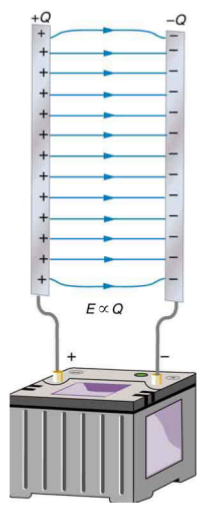
\includegraphics[width=0.25\textwidth]{figures/batt2.png}
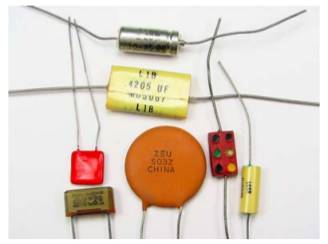
\includegraphics[width=0.5\textwidth]{figures/batt3.png}
\caption{\label{fig:batt2} A battery and a capacitor are not quite the same thing.}
\end{figure}
\end{frame}

\begin{frame}{Capacitance}
Parallel plate capacitor:
\begin{equation}
\boxed{
Q = \Delta V \left(\epsilon_0 \frac{A}{\Delta x}\right) = C\Delta V}
\end{equation}
How can we boost the charge?  Can we increase that $\epsilon_0$?  (It's a small number: $8.85 \times 10^{-12}$ N$^{-1}$ C$^2$ m$^{-2}$).  It turns out that by stuffing some insulating material between the plates \textit{boosts the capacitance...}
\end{frame}

\begin{frame}{Capacitance and Dielectrics}
Because \textit{dielectric} material reduces the field between the plates for the same charge, the voltage corresponding to that charge is reduced.  But that means \textit{higher capacitance}.
\begin{figure}
\centering
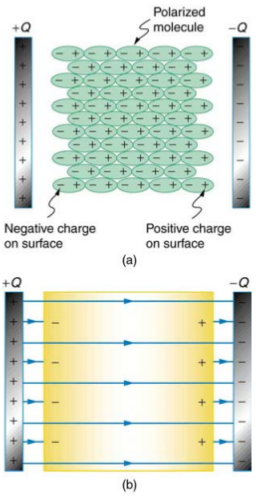
\includegraphics[width=0.25\textwidth]{figures/polar.png}
\caption{\label{fig:polar} Polarized dielectric.}
\end{figure}
\end{frame}

\begin{frame}{Capacitance and Dielectrics}
\begin{figure}
\centering
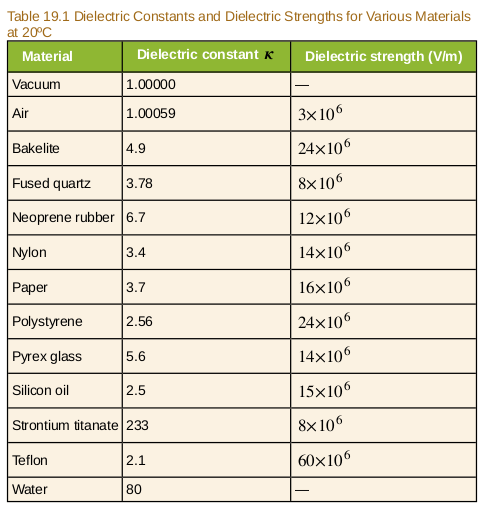
\includegraphics[width=0.5\textwidth]{figures/tableK.png}
\caption{\label{fig:tab} The middle column is the number by which $\epsilon_0$ is scaled up when dielectric is introduced.  We can't play this game indefinitely, because materials have a maximum electric field (third column) they can handle before they're ripped apart.}
\end{figure}
\end{frame}

\begin{frame}{Capacitance and Dielectrics}
\textbf{Group board exercise:} Suppose a capacitor (parallel plate) has area $A = 1$ cm$^2$ and separation $d = 1$ mm.  Using $\epsilon_0 = 8.85 \times 10^{-12}$ C$^2$ N$^{-1}$ m$^{-2}$, calculate the capacitance.  How much charge will be stored if we place 9 V across the capacitor?
\end{frame}

\begin{frame}{Capacitance and Dielectrics}
\textbf{Group board exercise:} Suppose we fill the capacitor with Teflon (see Tab. \ref{fig:tab}).  How much charge can we store with 9 V?
\end{frame}

\begin{frame}{Capacitance and Dielectrics}
\begin{figure}
\centering
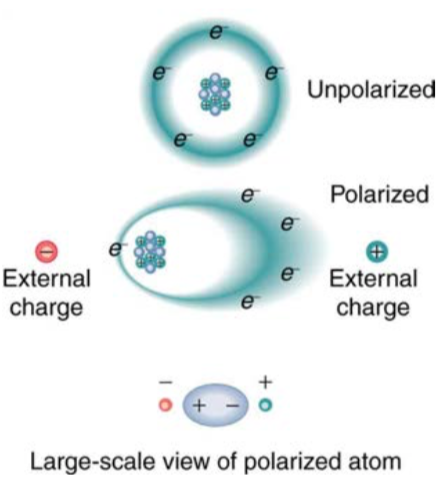
\includegraphics[width=0.5\textwidth]{figures/polar2.png}
\caption{\label{fig:polar2} Taking advantage of atomic structure in the dielectric.}
\end{figure}
\end{frame}

\begin{frame}{Capacitance and Dielectrics}
\begin{figure}
\centering
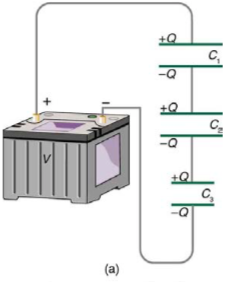
\includegraphics[width=0.4\textwidth]{figures/cap1.png} \hspace{0.2cm}
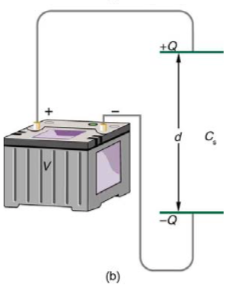
\includegraphics[width=0.4\textwidth]{figures/cap2.png}
\caption{\label{fig:cap} How do we compute the total capacitance of (a) such that we know the charge stored for a given voltage in (b)?}
\end{figure}
\end{frame}

\begin{frame}{Capacitance and Dielectrics}
\begin{itemize}
\item Notice that \textit{charge is conserved}, so $Q$ has to be the same on all capacitors
\item But that means the \textit{voltage} on the different capacitors has to obey
\begin{equation}
V = V_1 + V_2 + V_3
\end{equation}
and
\begin{align}
Q &= C_1 V_1 \\
Q &= C_2 V_2 \\
Q &= C_3 V_3
\end{align}
\end{itemize}
\end{frame}

\begin{frame}{Capacitance and Dielectrics}
\begin{itemize}
\item Combining equations:
\begin{align}
V &= \frac{Q}{C_{\rm total}} = \frac{Q}{C_1}+\frac{Q}{C_2}+\frac{Q}{C_3} \\
\frac{1}{C_{\rm total}} &= \frac{1}{C_1}+\frac{1}{C_2}+\frac{1}{C_3}
\end{align}
\item This is the capacitance for capacitors connected \textbf{in series}.
\end{itemize}
\end{frame}

\begin{frame}{Capacitance and Dielectrics}
\begin{figure}
\centering
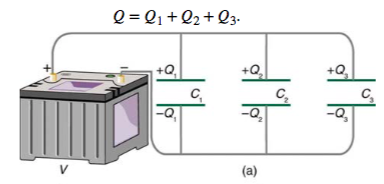
\includegraphics[width=0.4\textwidth]{figures/cap3.png} \hspace{0.2cm}
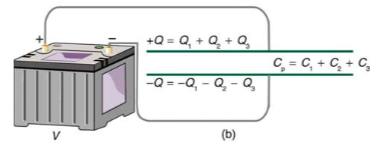
\includegraphics[width=0.4\textwidth]{figures/cap4.png}
\caption{\label{fig:cap2} How do we compute the total capacitance of (a) such that we know the charge stored for a given voltage in (b)?}
\end{figure}
\end{frame}

\begin{frame}{Capacitance and Dielectrics}
The result is:
\begin{equation}
C_{\rm total} = C_1+C_2+C_3
\end{equation}
This is the capacitance for capacitors connected \textbf{in parallel}.
\end{frame}

\section{Conclusion}

\begin{frame}{Unit 1 Summary}
\textbf{Reading: Chapters 18 and 19}
\begin{enumerate}
\item Charge, mass, the Coulomb force, and the gravitational force
\item Force fields
\item Electric potential and capacitance
\end{enumerate}
\end{frame}

\end{document}
